\documentclass[tc, manuscript]{copernicus}

\usepackage{booktabs}
\usepackage{multirow}
\usepackage{siunitx} 

\begin{document}

\title{Fountain scheduling strategies to improve water use efficiency of artificial
ice reservoirs (Icestupas)}

\def\Authors{Suryanarayanan Balasubramanian\,$^{1,2}$, Martin Hoelzle\,$^{1}$Roger Waser\,$^{3}$, $Martin Von
Burg^{3}\,$}

\def\Address{$^{1}$University of Fribourg, Department of Geosciences, Fribourg, Switzerland $^{2}$University of
Applied Sciences and Arts, Luzern, Switzerland} \def\corrAuthor{Suryanarayanan Balasubramanian}
\Author[1,2]{Suryanarayanan}{Balasubramanian}
\Author[1]{Martin}{Hoelzle}
\Author[3]{Roger}{Waser}
\Author[3]{Martin}{Von Burg}
\affil[1]{University of Fribourg, Department of Geosciences, Fribourg, Switzerland}
\affil[2]{Himalayan Institute of Alternatives, Ladakh, India}
\affil[3]{University of Applied Sciences and Arts, Luzern, Switzerland}

\correspondence{suryanarayanan.balasubramanian@unifr.ch}

\runningtitle{Scheduling AIR fountains}

\runningauthor{S. Balasubramanian}

\firstpage{1}

\maketitle

\begin{abstract}

  Artificial Ice Reservoir (AIR), often also called - Ice Stupa - are a climate adaptation strategy developed in
  the Indian Himalayas (Ladakh). With this technology, otherwise unused stream water is stored in large ice
  towers in winter. The surplus melt water that is then available in spring is used for satisfying irrigation
  water demands. Recent studies have shown that during construction of traditional AIRs over 75 \% of the water
  sprayed was lost. Therefore, fountain wastewater production have to be reduced to improve water use
  efficiency. Improved fountain scheduling was realized using an automation system that computes recommended
  discharge rates using real-time weather inputs and location metadata. During the winter of 2021-22, a
  traditional and an automated AIR were built in Guttannen, Canton of Berne, Switzerland with the main aim of
  comparing and quantifying the benefits of fountain scheduling through automation systems. The scheduled
  fountain produced similar ice volumes while consuming 79 \% lesser water than the unscheduled fountain.
  Simulations converting unscheduled fountains to scheduled fountains improved the water use efficiency of
  several traditional AIRs more than two fold. Overall, these results show that the automated construction
  strategy can increase the water use efficiency of AIRs without compromising their meltwater production.

\end{abstract}

\introduction

In some arid mountain regions the lack of water during the irrigation season is the main constraint on
agricultural production. Recently, an increasing need of irrigation water supply has prompted more than 30
villages in Ladakh, India to construct artificial ice reservoirs (AIRs) or icestupas. These AIRs are
traditionally constructed by diverting springs or glacial streams into fountain spray systems via
embankments and pipelines. However, there is a large variability associated with this water supply due to the
local weather influences and discharge rate of the chosen location and fountain respectively. 

Previous studies \citep{balasubramanianInfluenceMeteorologicalConditions2022,
oerlemansBriefCommunicationGrowth2021} have already quantified the meteorological influences on AIR volume
evolution by comparing several AIRs built in India and Switzerland. The results revealed the high sensitivity of
AIR volume evolution on the fountain characteristics. Moreover, it was found that all the AIRs constructed
suffered from very high water losses due to excessive fountain discharge input. 

A straightforward solution to this issue is to reduce the fountain discharge input but it is challenging to
implement it in practice. For example, in the case of the Indian AIR, the model estimates that water use
efficiency can be increased by just reducing the fountain discharge rate by half. However, in practice, this
strategy would have further increased the number of fountain freezing events due to much lower water velocities
in the pipeline. Moreover, the Indian AIR discharge rate was lowered temporally due to increase in fountain
height from 5 to 9 m. Therefore, any reduction in initial discharge rate would have triggered a fountain
freezing event before the fountain height could be increased to 9 m.

An optimum construction strategy, therefore, should prevent fountain freezing events while maintaining high
water use efficiency. Fountain freezing events can be prevented if the pipeline water temperature is maintained
above 0 $\degree C$ and the discharge is not lowered below a critical threshold. Typical solutions to maintain
pipeline water temperature given pipeline dimensions are to bury or drain the pipeline. Burying the pipeline at
a sufficient depth can reduce the influence of atmospheric conditions on the pipeline water temperature. Even
though this method is ideal, it can quickly get expensive depending on the length of the pipeline and the frost
depth. Therefore, such an effort is warranted only in the case of a permanent construction location.
Comparatively, draining the pipeline when the fountain is not active is a much cheaper strategy. Fountain
discharge rate is lowered every time the fountain height increases. Therefore, a critical discharge rate needs
to be set beyond which fountain height should not be increased. Moreover, both these strategies can be combined
with fountain scheduling methods to achieve reduced watering volumes for AIR construction systems. 

Proper fountain scheduling requires answers to two questions: 
(a) When should the water be turned on and off ?
(b) How much water should be sprayed ? 

For answering these questions, knowledge of surface freezing rates is important . Surface freezing rates can be
calculated by means of the full energy balance model developed in
\cite{balasubramanianInfluenceMeteorologicalConditions2022}. This model can be forced with either historical
weather data or real-time weather data to produce recommended discharge rates. We further approximate the model
by including two kinds of assumptions that are considerate for the limited water availability or the favourable
weather windows respectively.

However, manually adjusting the fountain discharge rate is unrealistic. Firstly, constant adjustments of
discharge rates in response to the significant diurnal and seasonal variations of the freezing rates is
impractical. Secondly, frequent pipeline water drainage required to prevent freezing events during critical weather
windows is unfeasible. Therefore, operation of scheduled fountains via automation systems is preferred.

The present study builds upon previous work \citep{balasubramanianInfluenceMeteorologicalConditions2022,
oerlemansBriefCommunicationGrowth2021}, in order to quantify the influence of different fountain scheduling
strategies on the mass and energy balance of AIRs with identical meteorological conditions. The main interest in
using model results is to simulate fountain schedules relative to constraints in favourable weather windows and
water availability. The fountain scheduling strategies are evaluated from the relative water use efficiency and
maximum ice volume produced during the study period. The specific objectives of this paper include the mass and
energy balance comparison of fountain scheduling strategies, presentation of the automation system, and examples
of its application to the computation of fountain scheduling strategies.

\section{Study site and data}

The Guttannen site (46.66 $\degree$N, 8.29 $\degree$E) is situated in the Berne region, Switzerland and has an
altitude of 1047 $m$ a.s.l. In the winter (Oct-Apr), mean daily minimum and maximum air temperatures vary
between -13 and 15 $\degree C$. Clear skies are rare, averaging around 7 days during winter. Daily winter
precipitation can sometimes be as high as 100 $mm$. These values are based on 30 years of hourly weather model
simulations \citep{guttannen}. Two AIRs were constructed by the Guttannen Bewegt Association, the University of
Fribourg and the Lucerne University of Applied Sciences and Arts during the winters of 2021-22 using a
traditional and an automated construction strategy.

\begin{figure}[t]
\includegraphics[width=8.3cm]{Figures/2AIRs.jpg}
\caption{Automated and traditional AIRs  at Guttannen on February 6, 2022. Picture credits: Daniel Bürki}
\label{fig:2AIR} 
\end{figure}

The automated and the traditional AIRs were constructed adjacent to each other as shown in Fig. \ref{fig:2AIR}.
This ensured both AIRs shared the same water source and similar weather conditions. In addition, a webcam
guaranteed a continuous survey of the automated AIR.   

In the traditional strategy, tree branches were laid covering the fountain pipe to initiate and speed up the ice
cone formation process. The fountain discharge was maintained at maximum and its height was increased from 3 to
6\,$m$ during the construction period.

In the automated strategy, only the fountain pipe was placed before the water spray started. A programmed
automation system controlled the fountain discharge rate during the whole winter season using real time weather
input and several control parameters, which could be tested and controlled via a user interface. 

\subsection{Meteorological data}

Air temperature, relative humidity, wind speed, pressure, longwave, shortwave direct and diffuse radiation are
required to calculate the surface energy balance of an AIR (see Fig. \ref{fig:aws}). The construction period
starts when the fountain was first switched on and ends when the AIR melts completely. These two dates are denoted
as start and expiry dates henceforth.

\begin{figure*}[t]
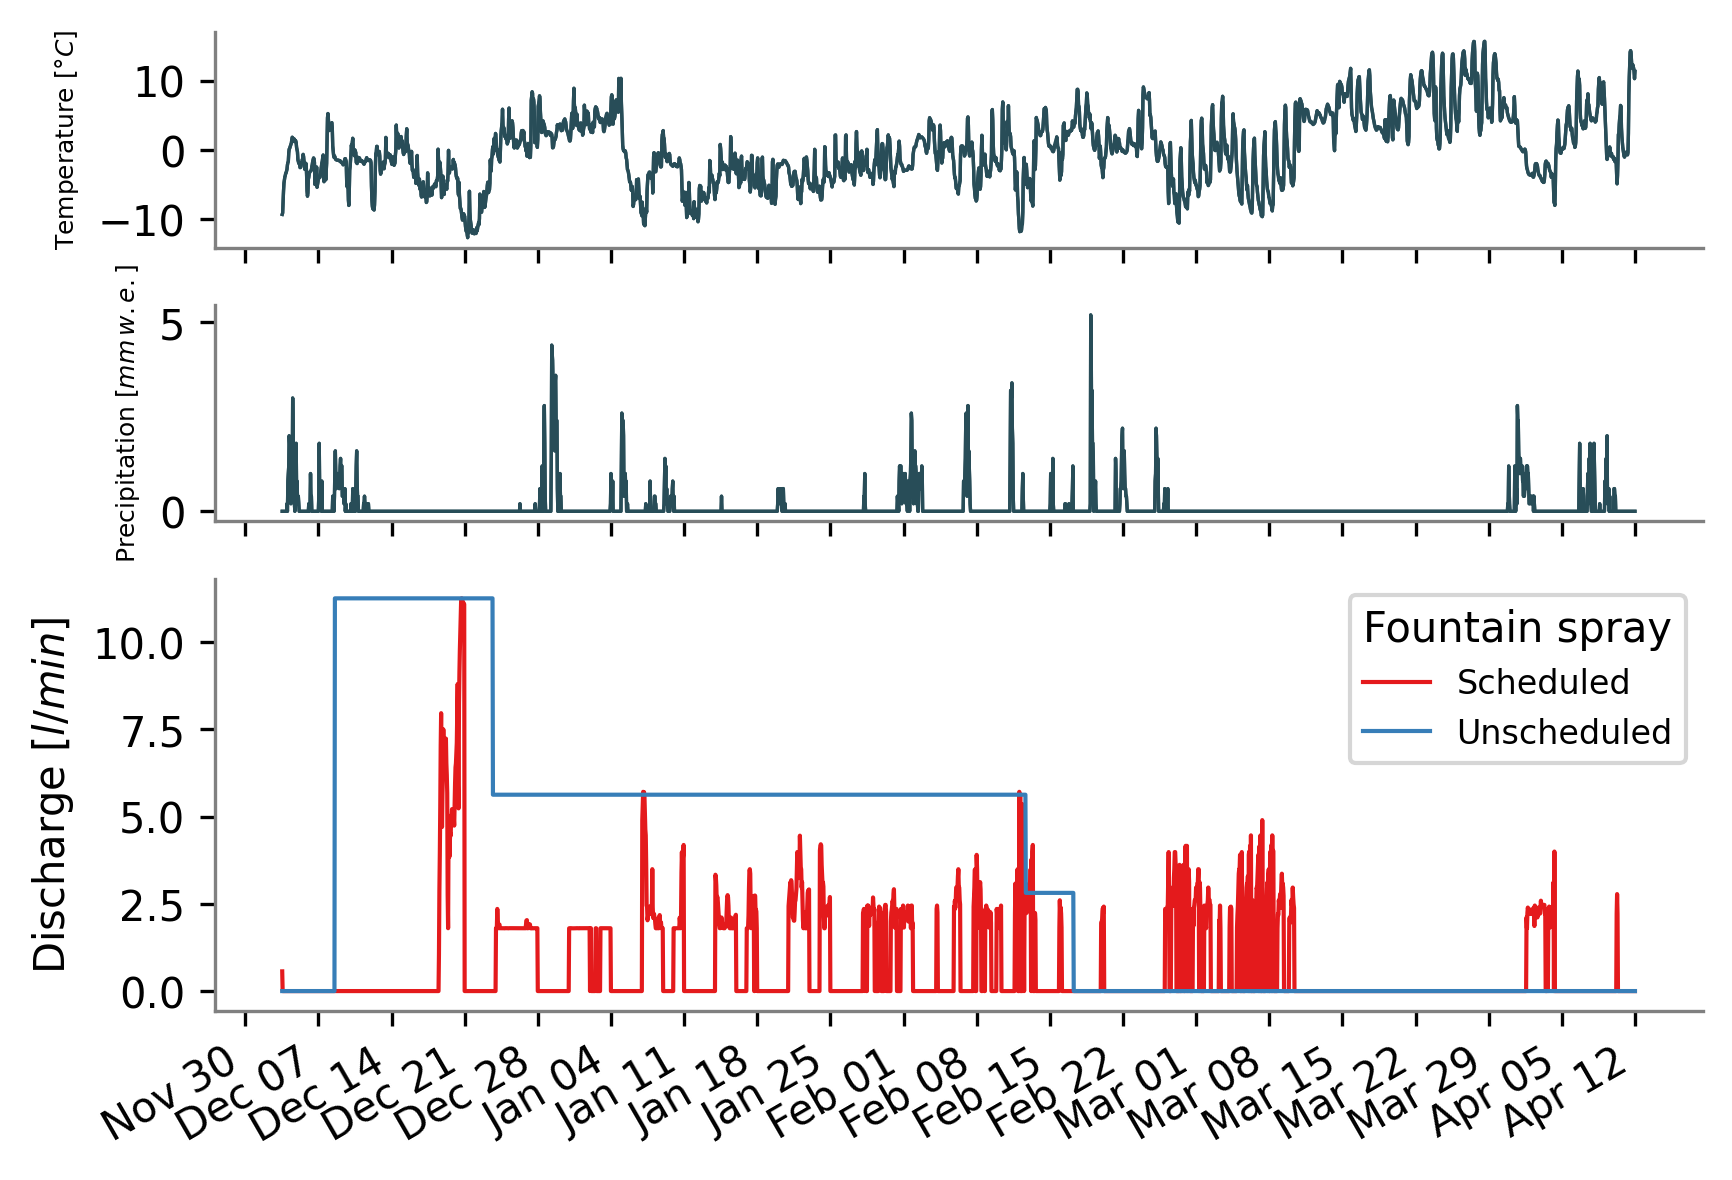
\includegraphics[width=12cm]{Figures/data.png}
\caption{Temperature, precipitation and discharge measurements at the Guttannen construction site}
\label{fig:aws} 
\end{figure*}

The weather data source was an automatic weather station (AWS) located around 20 m away as shown in Fig.
\ref{fig:2AIR}. Less than 0.4 \% of the data was found to be missing and these were filled by linear
interpolation. 

\subsection{Fountain observations}

We define the fountain used through its four attributes namely, spray radius ($r_F$), discharge rate ($Q_F$),
height ($h_F$) and water temperature ($T_F$). Spray radius denotes the maximum radius of impact of the fountain
water droplets. Discharge rate represents the discharge rate of the water in the fountain pipeline. Height
denotes the height of the fountain pipeline installed. Fountain water temperature is the temperature of the
water droplets produced by the fountain.

The spray radius was estimated from the mean AIR circumference measured in the drone surveys during the fountain
runtime. The discharge rate and water temperature of the scheduled fountain was measured by the automation
system but no such datasets were recorded for the unscheduled fountain. The unscheduled fountain was operated at
the maximum discharge rate using the same water source. Therefore, the maximum recorded discharge rate and water
temperature dataset of the scheduled fountain was used to estimate the corresponding variables of the
unscheduled fountain. The discharge rate of both fountains decreased with increase in its fountain height. We
observed a reduction in the scheduled fountain's maximum discharge rate by a factor of two whenever the height
was increased by a meter. The same reduction in magnitude was also applied for the unscheduled fountain's
discharge rate whenever pipeline height increase events occurred. 

\subsection{Drone surveys}

Several photogrammetric surveys were conducted on the traditional and the automated AIRs. The details of these
surveys and the methodology used to produce the corresponding outputs are explained in
\cite{balasubramanianInfluenceMeteorologicalConditions2022}. The digital elevation models (DEMs) generated from
the obtained imagery were analysed to document the spray radius, the surface area and the volume of the ice
structures. Even though the number of drone flights were identical for both AIRs, fewer successful volume
observations were possible for the automated AIR as shown in Table \ref{tab:uav}. This was because the DEMs
generated for the automated AIR could not georeference the automated AIR's snow covered surface. Since the
traditional AIR was steeper, its surface revealed ice patches that could be georeferenced. The number of drone
surveys conducted for the traditional and the automated AIRs were 8 and 6, respectively (see Table). 

\begin{table}
	\centering
	\caption{ Summary of the drone surveys}
	\label{tab:uav}
	\begin{tabular}{@{}|llllll|@{}}
		\toprule
		\textbf{}              & \textbf{No.} & \textbf{Date} & \textbf{Volume} & \textbf{Radius} & \textbf{Surface Area} \\ \midrule
		\multicolumn{1}{|l|}{\multirow{8}{*}{\rotatebox[origin=c]{90}{Traditional}}}
		                       & 1            & Dec 23, 2021  & 17 $m^{3}$     & 2.9 $m$
		                       & 47 $m^{2}$                                                                      \\
		\multicolumn{1}{|l|}{} & 2            & Jan 3, 2022  & 22 $m^{3}$     & 3.4 $m$
		                       & 61 $m^{2}$                                                                      \\
		\multicolumn{1}{|l|}{} & 3            & Jan 22, 2022   & 35 $m^{3}$     & 4 $m$
		                       & 79 $m^{2}$                                                                      \\
		\multicolumn{1}{|l|}{} & 4            & Feb 6, 2022  & 44 $m^{3}$     & 4.2 $m$
		                       & 86 $m^{2}$                                                                      \\
		\multicolumn{1}{|l|}{} & 5            & Feb 20, 2022  & 43 $m^{3}$     & 4.3 $m$
		                       & 86 $m^{2}$                                                                      \\
		\multicolumn{1}{|l|}{} & 6            & Mar 19, 2022  & 33 $m^{3}$     & 4.4 $m$
		                       & 84 $m^{2}$                                                                      \\
		\multicolumn{1}{|l|}{} & 7            & Mar 26, 2022  & 24 $m^{3}$     & 4.3 $m$
		                       & 74 $m^{2}$                                                                      \\
		\multicolumn{1}{|l|}{} & 8            & Apr 12, 2022  & 11 $m^{3}$     & 3.5 $m$
		                       & 50 $m^{2}$                                                                      
		\\\midrule
		\multicolumn{1}{|l|}{\multirow{6}{*}{\rotatebox[origin=c]{90}{Automatic}}}
		                       & 1            & Dec 23, 2021  & 35 $m^{3}$      & 4.3 $m$
		                       & 73 $m^{2}$                                                                       \\
		\multicolumn{1}{|l|}{} & 2            & Jan 3, 2022   & 32 $m^{3}$      & 4.4 $m$
		                       & 81 $m^{2}$                                                                       \\
		\multicolumn{1}{|l|}{} & 3            & Feb 20, 2022   & 60 $m^{3}$      & 5.3 $m$
		                       & 105 $m^{2}$                                                                       \\
		\multicolumn{1}{|l|}{} & 4            & Mar 19, 2022   & 28 $m^{3}$      & 3.7 $m$
		                       & 57 $m^{2}$                                                                       \\
		\multicolumn{1}{|l|}{} & 5            & Mar 26, 2022   & 19 $m^{3}$      & 3.7 $m$
		                       & 53 $m^{2}$                                                                       \\
		\multicolumn{1}{|l|}{} & 6            & Apr 12, 2022   & 7 $m^{3}$      & 2.5 $m$
		                       & 53 $m^{2}$                                                                       \\
		\bottomrule
	\end{tabular}

\end{table}

\section{Methods}

\subsection{Automation system}

\subsubsection{Automation hardware}

The automation hardware consists of an AWS, flowmeter, control valve, drain valves, air valves, fountain,
pipeline and a logger. The logger feeds the AWS data to the automation software and informs the recommended
discharge rate to the flowmeter. The flowmeter adjusts the control valve to match the recommendation. However,
the recommended discharge rate is ignored if any of the termination criterion are valid. The termination
criterion prevent water loss and fountain freezing events. In case a termination criteria is valid, the drain
and air valves allow the removal of water from the pipeline and entry of air in the pipeline respectively.

\subsubsection{Automation software}

Any construction location can either be constrained by the available water supply or the duration of favourable
weather windows for fountain operation. If the respective location has limited water supply then the fountain
scheduling strategy should be optimised for high water use efficiency (WUE). But if the location is limited by
the time period when the fountain can function then the scheduling strategy should be optimised for high ice
volumes (ICV).

Accordingly, we introduce two kinds of approximations in the automation software that optimise for the ICV and
WUE objective respectively. We approximate the expected (a) AIR shape using its slope parameter, (b) AIR surface
properties using its surface albedo and (c) weather conditions using the cloudiness parameter. The model
assumptions overestimate and underestimate the freezing rate for the ICV and WUE objectives respectively. These
assumptions are summarised in Table \ref{tab:assumptions}. 

\begin{table}[]
\centering
\caption{Assumptions introduced to simplify the model.}
\label{tab:assumptions}
\begin{tabular}{@{}lllll@{}}
\toprule
\textbf{Estimation of} & \textbf{Symbol} & \textbf{ICV Assumptions} & \textbf{WUE Assumptions} & \\ \midrule
\multicolumn{1}{|l}{AIR slope}        & $s_{cone}$ & $ 1 $ & $0$ & \multicolumn{1}{l|}{} \\ \midrule
\multicolumn{1}{|l}{Albedo} & $\alpha$ & $\alpha_{snow}$ & $\alpha_{ice}$ & \multicolumn{1}{l|}{} \\\midrule 
\multicolumn{1}{|l}{Cloudiness}  & $cld$ & $0$ & $1$ & \multicolumn{1}{l|}{} \\ \bottomrule
\end{tabular}
\end{table}

We apply the assumptions described in Table \ref{tab:assumptions} on the one-dimensional description of energy
fluxes as used in \cite{balasubramanianInfluenceMeteorologicalConditions2022} to obtain the rate of change of
AIR ice mass as follows: 

\begin{equation}
  \frac{\Delta M_{ice}}{\Delta t}  =  (\frac{q_{SW} + q_{LW} + q_{S} + q_{F} + q_{R} + q_{G} - q_{T}}{L_F} + \frac{q_{L}}{L_V} ) \cdot A_{cone}
	\label{eqn:auto}
\end{equation}

Upward and downward fluxes relative to the ice surface are positive and negative, respectively. The first term
represents the mass change rate due to freezing of the fountain water and melting of the ice. $q_{SW}$ is the
net shortwave radiation; $q_{LW}$ is the net longwave radiation; $q_{L}$ and $q_{S}$ are the turbulent latent
and sensible heat fluxes; $q_{F}$ is the fountain discharge heat flux; $q_{R}$ is the rain water heat
flux; $q_{G}$ is the ground heat flux; $q_{T}$ is the temperature heat flux and $A_{cone}$ is the area of the
AIR surface. The derivation of these individual terms using the assumptions are discussed in the Appendix.

Equation \ref{eqn:auto} is implemented in the automation system through a user interface that enables input of
the spray radius, altitude, latitude and longitude of the construction location. Once switched on, the
automation system regulates the fountain discharge rate based on the recommended discharge rate. The recommended
discharge rate is equal to the ice mass change rate. However, certain termination criterias override the
discharge rate recommendation and drain the pipeline to prevent water loss or fountain freezing events, namely: 

\begin{itemize}

\item High water loss is assumed if wind speed greater than critical wind speed.

\item High risk of fountain freezing event is assumed if temperature lower than fountain freezing temperature.

\item High risk of fountain freezing event is assumed if $\frac{\Delta M_{ice}}{\Delta t}$ is lower than minimum fountain discharge rate. 

\item Fountain freezing events are assumed if $Q_F = 0$ for at least 20 seconds and the pipeline is drained as a
  consequence.

\item Pipeline leakage is assumed if $Q_F$ is greater than maximum fountain discharge rate.

\end{itemize}

\subsection{Model updates}

The model had to be made more sensitive to fountain discharge rate feedback in order to compare the volume
evolution of the automated and the traditional AIRs. This was done by introducing better parametrisations of
fountain water temperature and surface albedo. 

In the previous version of the model, the fountain water temperature ($T_F$) was estimated as a constant
parameter. However, in reality, the water droplets cool to 0 C during their flight time under subzero
conditions. Therefore, the fountain water temperature was instead determined as follows:

\begin{equation}
	T_{F} = \left\{ \begin{array}{ll}
		0 & \textit{ if } T_{a} < 0 \\
		T_{F} & \textit{ otherwise}
	\end{array} \right.
\end{equation}

In the previous version of the model, fountain discharge events reset surface albedo to that of the ice albedo.
This assumption limits the accuracy of the model especially for the Automated AIR where there were several
fountain discharge events of short durations. Therefore, we assumed that discharge events instead
increase the albedo decay rate ($\tau$) by a scaling factor equal to $\frac{\alpha_{snow}}{\alpha_{ice}}$.

Additionally, both the AIRs experienced many precipitation events. Therefore, it was no longer accurate to
assume AIR density ($\rho_{AIR}$) to be a constant. We instead parameterised AIR density $\rho_{AIR}$ as follows:

\begin{equation}
  \rho_{AIR} = \frac{M_{F} + M_{dep} + M_{ppt}}{(M_{F} + M_{dep})/\rho_{ice} + M_{ppt}/\rho_{snow}}
\end{equation}

where $M_F$ is the cumulative mass of the fountain discharge; $M_{ppt}$ is the cumulative precipitation; $M_{dep}$ is the cumulative accumulation through water vapour deposition; $\rho_{ice}$ is the ice density (917 $kg\,m^{-3}$) and $\rho_{snow}$ is the density of wet snow (300 $kg\,m^{-3}$) taken from
\cite{cuffeyPhysicsGlaciers2010} .

Rain events were not considered in the previous version of the model but they occur in our experiment.
Accordingly, the model algorithm was updated to accomodate for these events. The influence of rain events on the
albedo and the energy balance was assumed to be similar to that of discharge events. However, the water
temperature of a rain event was assumed to be equal to the air temperature. Accordingly, the heat flux generated
due to a rain event was equal to:

\begin{equation}
  q_{R} = \frac{\Delta M_{ppt} \cdot c_{water} \cdot T_{a}}{\Delta t \cdot A_{cone}}
\end{equation}

\subsection{Calibration and Validation}

The model parameters were calibrated to the median values of the ranges presented in
\cite{balasubramanianInfluenceMeteorologicalConditions2022}.

We performed the validation of the model on the traditional and automated AIRs by evaluating the root mean
squared error (RMSE) between ice volume estimates and measurements. 

The performance of the ICV and WUE versions of the physical model was assessed by comparing correlation of its
discharge rate estimates with the validated freezing rate of the calibrated physical model.

\subsection{Fountain characteristics}

The influence of the fountain characteristics namely, its aperture diameter ($dia$) and height ($h$) on the
the discharge of the fountain ($Q$) can be determined from the Bernoulli equation :

\begin{equation}
  \label{eqn:fountain}
  P_{i} + \rho_{water} \cdot g \cdot h_{i} + 1/2 \cdot \rho_{water} \cdot v_{i}^2 = P_{f} + \rho_{water} \cdot g
  \cdot h_{f} + 1/2 \cdot \rho_{water} \cdot v_{f}^2
\end{equation}

where $P$ is the pressure loss caused by the fountain, $\rho_{water}$ is the density of water and $v$ is the
velocity of the fountain water droplets. The subscripts $i$ and $f$ refer to the initial and final states of the
system. $v$ can be determined from the discharge rate $Q$ through the mass conservation equation as 

\begin{equation}
 v = 4 \cdot Q/(\pi \cdot dia^2)
\end{equation}

Combining the above two equations we get the final discharge $Q_f$ after a height change from $h_i$ to $h_f$ to be :

\begin{equation}
  \label{eqn:discharge}
  Q_f = \sqrt{Q_i^2 + 2 \cdot g \cdot (h_f-h_i) \cdot (\pi \cdot dia^2/4)^2}
\end{equation}


\section{Results}

\subsection{Energy balance model validation}

The volume estimation for the automated and traditional AIR had an RMSE of 7 $m^3$ and 5 $m^3$ with the ice
volume observations respectively. The estimated and measured AIR ice volumes are shown in Fig.
\ref{fig:validation}.
 
\begin{figure*}[t] 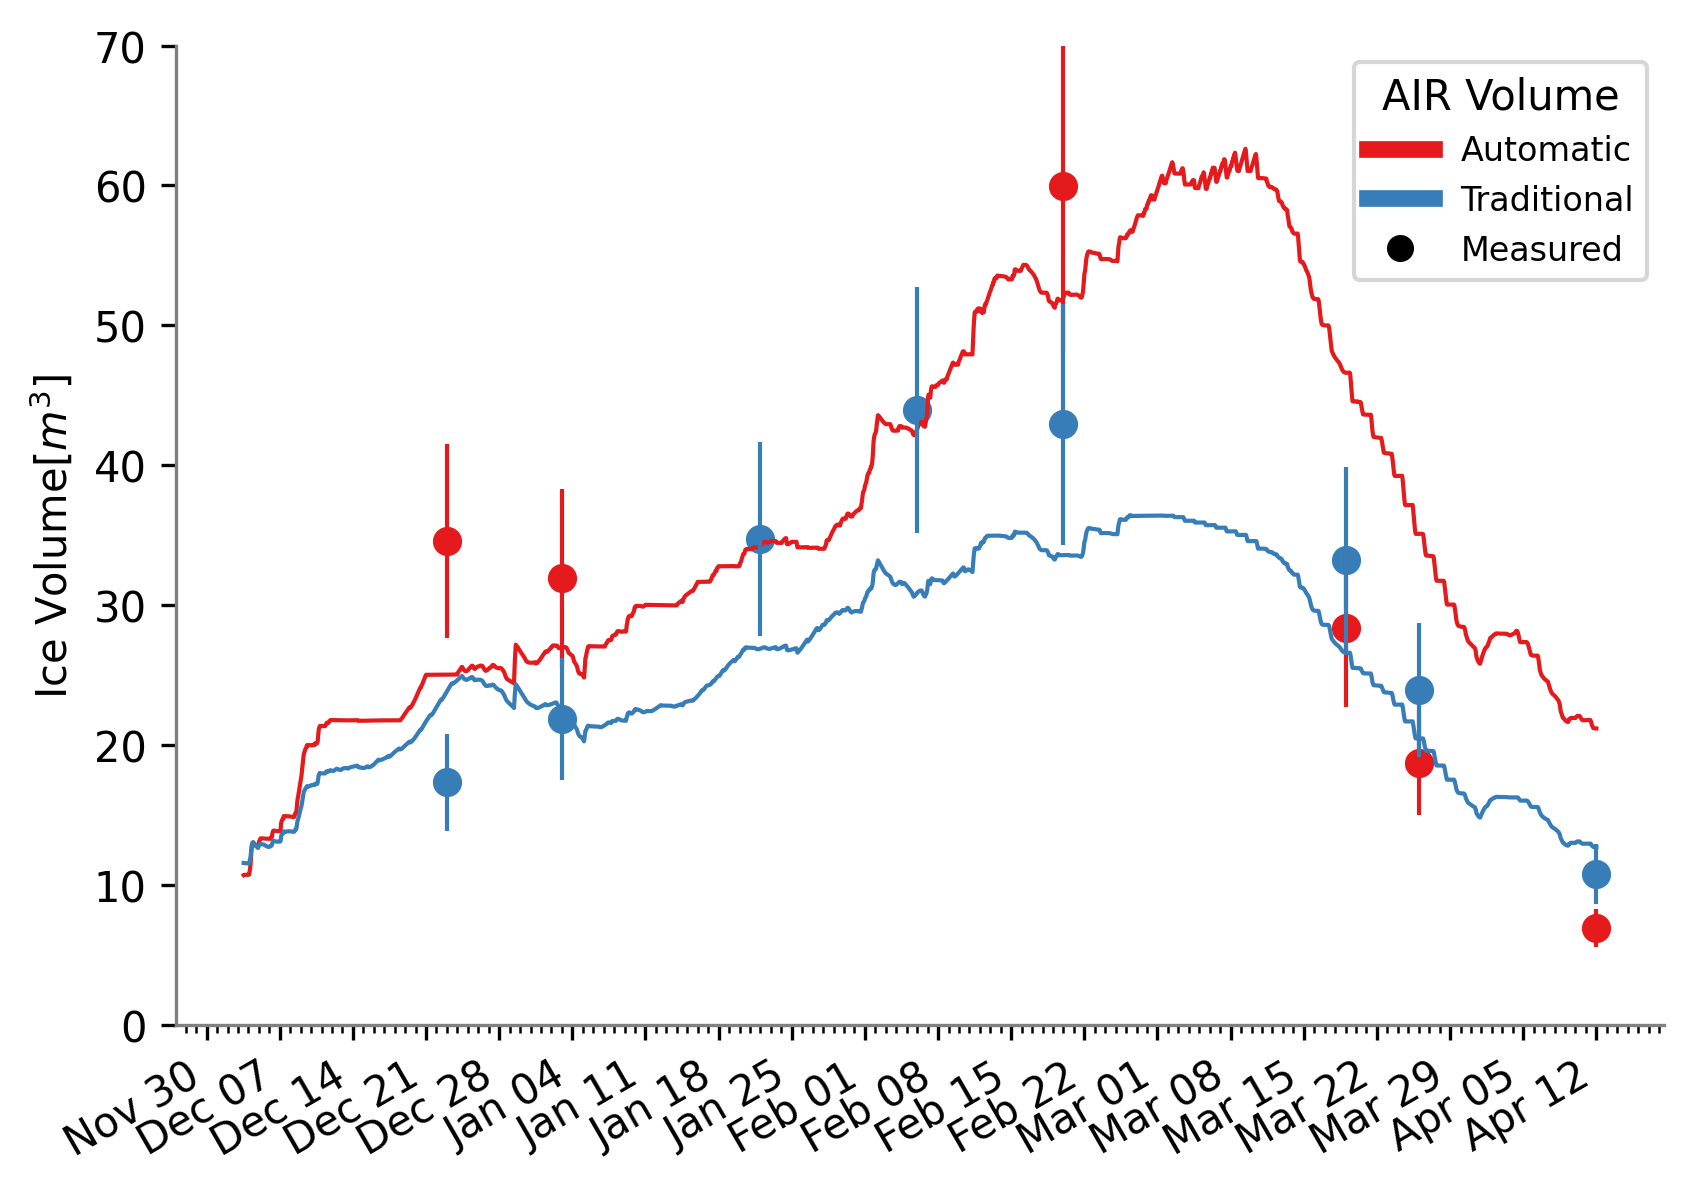
\includegraphics[width=12cm]
  {Figures/validation.png} 
  \caption{Ice volume validation of the scheduled and unscheduled fountain construction strategies.} 
\label{fig:validation} 
\end{figure*}

\subsection{Scheduled discharge rate estimation}

We found that the simplified energy balance model estimated the freezing rate of the unscheduled fountain with a
correlation around 0.6 and a RMSE less than 0.6 $l/min$ and 1.6  $l/min$ for the WUE and ICV objectives
respectively. The ICV scheduled fountain overestimated the freezing rate 90 \% of the construction duration
whereas the WUE scheduled fountain underestimated the freezing rate 80 \% of the construction duration.

\subsection{Comparison of AIR construction strategies}

\begin{figure*}[t]
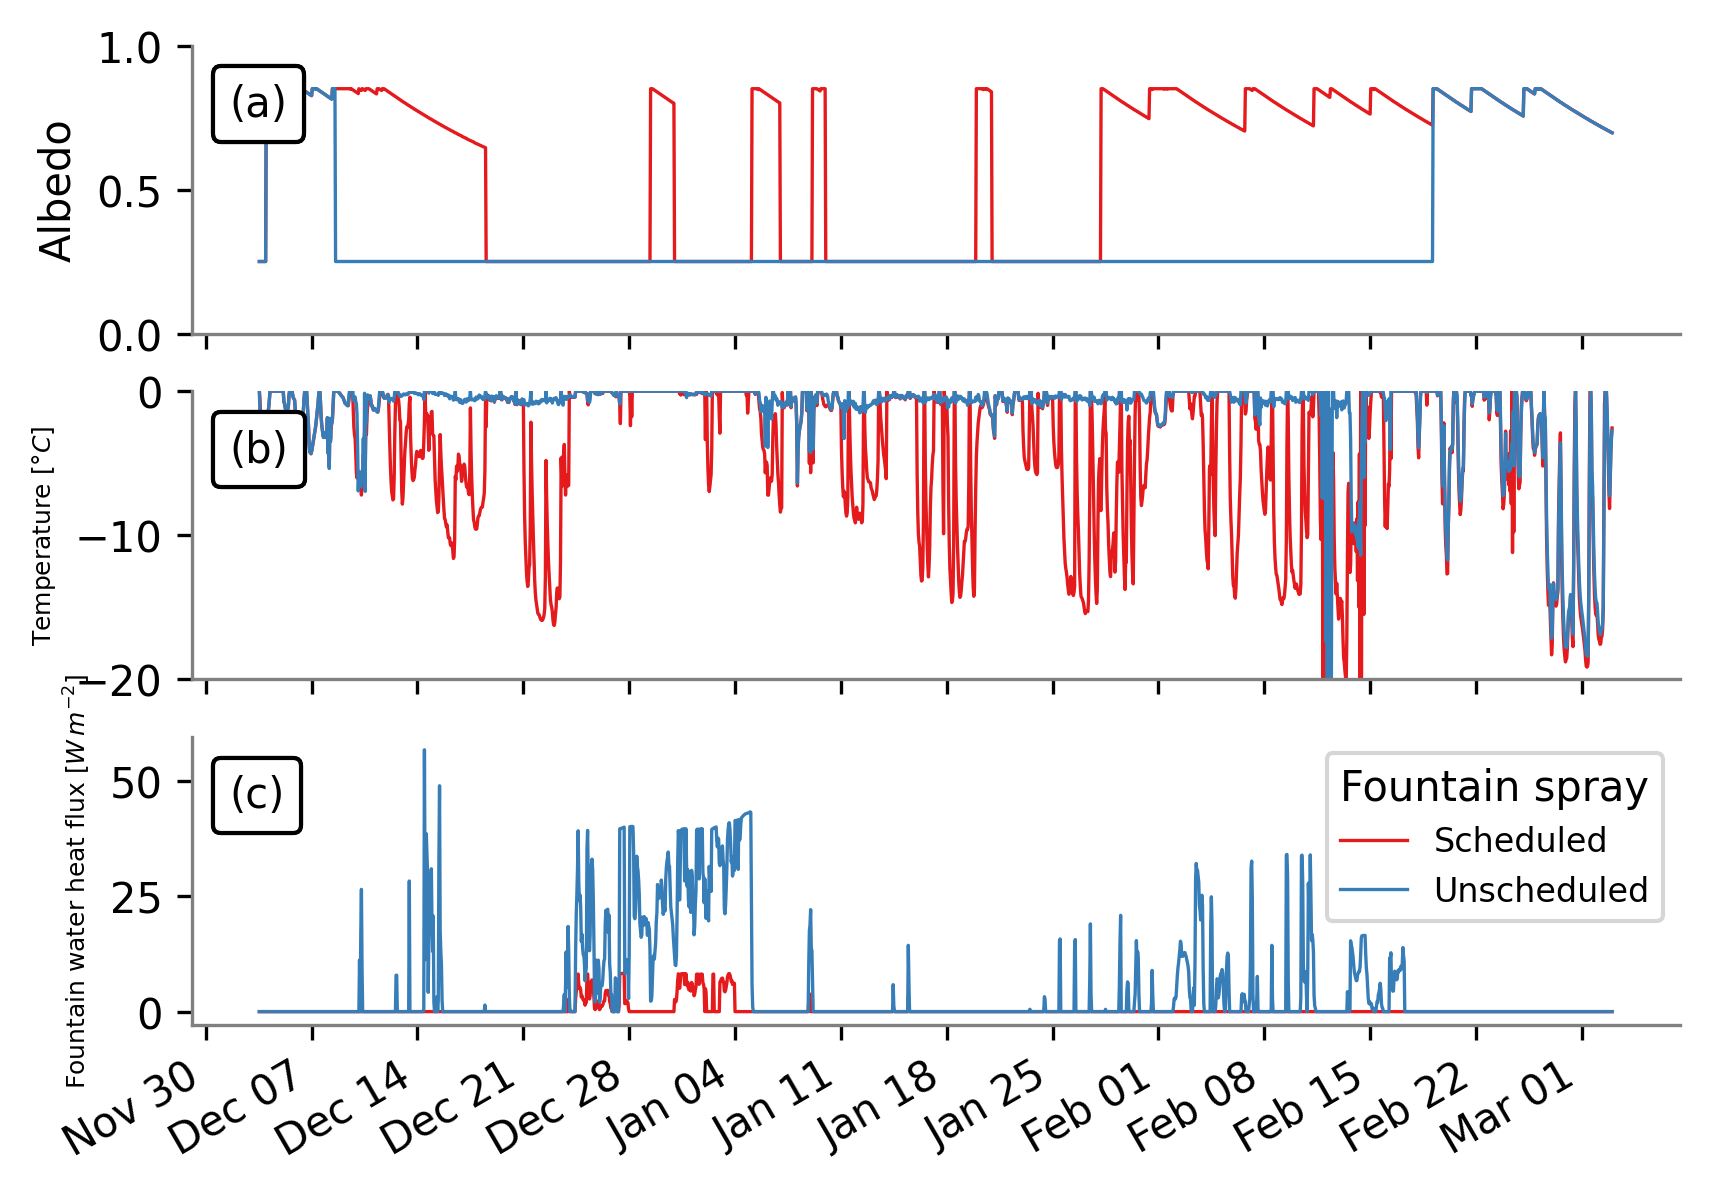
\includegraphics[width=12cm]{Figures/dis_processes.png}
\caption{Surface albedo (a) and fountain discharge heat flux (b) showed significant variations between the two
  AIRS due to the differences in their discharge rate.}
\label{fig:dis_processes}
\end{figure*}

Table \ref{tab:mb} shows how the different fountain scheduling strategies influence the mass and energy balance
of the respective AIR. The largest difference between the mass balance of the unscheduled and scheduled
fountains were found to be in the fountain discharge input and fountain wastewater output. This was expected
since the unscheduled fountain's discharge duration was 2 times higher than the scheduled fountain.

To understand how the different scheduling strategies influence the rest of the mass balance output, we discuss
the influence of fountain discharge on the surface mass and energy balance. During fountain spray, the AIR
surface is affected in the following two ways, namely, (a) its albedo dampens to ice albedo and (b) it absorbs
the heat energy of the fountain water droplets. These two processes are the cause of the difference in the mass
and energy balance distribution shown in Table \ref{tab:mb}. The temporal variation of the magnitude of these
processes are shown in Fig. \ref{fig:dis_processes}. 

To understand the overall impact of the radiation fluxes (longwave and shortwave) and the turbulent fluxes
(sensible and latent) on the freezing and melting energies, we sum their respective energy turnover by taking
into account the sign of their mean energy during the study period (see Table \ref{tab:mb}). A negative sign
indicates that the corresponding energy flux increased/decreased the freezing/melting energy respectively.  The
radiation fluxes contributed -6 \% and 4 \% to the freezing and melting energies for the traditional and
automated AIR, respectively.  Similarly, the turbulent fluxes contribute -10 \% and -9 \% to the freezing
energies for the traditional and automated AIR, respectively. The fountain water and ground heat flux contribute
11 \% and 3 \% to the melting energies for the traditional and automated AIR, respectively. 

There is a considerable difference in the contribution of the shortwave radiation due to the effect of process
(a). Even though the traditional AIR was active for a much longer duration, the frequent snowfall events
counteracted the albedo feedback of its fountain discharge. However, the albedo of the automated AIR was
significantly impacted by late fountain spray events particularly in the month of March as shown in Fig.
\ref{fig:dis_processes}.

Similarly, the fountain discharge heat flux for the traditional AIR is enhanced due to process (b). The higher
quantity of the unscheduled fountains and its longer duration are responsible for the 10 fold increase in its
fountain discharge heat flux.


\begin{table}
	\centering
	\caption{Summary of the mass balance, energy balance, fountain and AIR characteristics estimated at the end of the respective
  simulation duration for the automated and the traditional AIRs}
	\label{tab:mb}
	\begin{tabular}{@{}|llllll|@{}}
		\toprule
		\textbf{}              & \textbf{Name}                   & \textbf{Symbol} & \textbf{Traditional} & \textbf{Automated} &
		\textbf{Units}                                                                                                       \\ \midrule
		\multicolumn{1}{|l|}{\multirow{3}{*}{\rotatebox[origin=c]{90}{Input}}}
		                       & Fountain discharge              & $M_F$           & \num{6.8e5}   & \num{1.4e5}     & $kg$  \\
		\multicolumn{1}{|l|}{} & Snowfall                        & $M_{ppt}$       & \num{1.1e4}   & \num{1.5e4}   & $kg$  \\
		\multicolumn{1}{|l|}{} & Deposition                      & $M_{dep}$       & \num{8.8e2}   & \num{1.2e3}     & $kg$  \\ \midrule
		\multicolumn{1}{|l|}{\multirow{4}{*}{\rotatebox[origin=c]{90}{Output}}}
		                       & Meltwater                       & $M_{water}$     & \num{3.3e4} & \num{4.2e4}   & $kg$  \\
		\multicolumn{1}{|l|}{} & Ice                             & $M_{ice}$       & \num{1.4e4} & \num{1.3e4}    & $kg$  \\
		\multicolumn{1}{|l|}{} & Sublimation                     & $M_{sub}$       & \num{2.6e3} & \num{3.0e3}     & $kg$  \\
		\multicolumn{1}{|l|}{} & Fountain wastewater             & $M_{waste}$     & \num{6.6e5} & \num{1.1e5}     & $kg$  \\ \midrule
		\multicolumn{1}{|l|}{\multirow{6}{*}{\rotatebox[origin=c]{90}{Energy Balance}}}

                           & Shortwave radiation             &  $q_{SW}$       & $29$  & $39$ & \% \\
		\multicolumn{1}{|l|}{} & Longwave radiation              &  $q_{LW}$       & $-35$  & $-35$ & \% \\
		\multicolumn{1}{|l|}{} & Sensible heat                   &  $q_{S}$        & $8$   & $8$ & \% \\
		\multicolumn{1}{|l|}{} & Latent heat                     &  $q_{L}$        & $-18$  & $-17$ & \% \\
		\multicolumn{1}{|l|}{} & Fountain discharge heat         &  $q_{F}$        & $10$  & $1$     & \% \\
		\multicolumn{1}{|l|}{} & Ground heat                     &  $q_{G}$        & $1$   & $2$     & \% \\\midrule
		\multicolumn{1}{|l|}{\multirow{5}{*}{\rotatebox[origin=c]{90}{Fountain}}}

                           & Spray Radius                    &  $r$            & 4.8           & 4.1           & $m$ \\
		\multicolumn{1}{|l|}{} & Aperture Diameter               &  $dia$          & 5             & Higher        & $mm$ \\
		\multicolumn{1}{|l|}{} & Pressure Loss                   &  $P$            & 0.43          & Lower         & $bars$ \\
		\multicolumn{1}{|l|}{} & Critical discharge rate         &  $Q_{crit}$     & $5$           & Lower         & $l/min$ \\
		\multicolumn{1}{|l|}{} & Minimum discharge rate          &  $Q_{min}$      & $2$           & N.A.          & $l/min$ \\\midrule
		\multicolumn{1}{|l|}{\multirow{2}{*}{\rotatebox[origin=c]{90}{AIR}}}

		                       & Maximum Ice Volume              &                 & 47            & 63            & $m^{3}$ \\
		\multicolumn{1}{|l|}{} & Water Use Efficiency            &                 & 6             & 32            & \% \\\midrule
	\end{tabular}
\end{table}

\subsection{Estimation of fountain characteristics}

\subsubsection{Aperture diameter}

The maximum discharge rate of the scheduled fountain was reduced from $Q_i$ =  13 $l/min$ to $Q_f$ = 11 $l/min$
when the fountain height was raised from  $h_i$ = 3 $m$ to $h_f$ = 4 $m$. Inputting the corresponding values in
Eqn. \ref{eqn:fountain_min}, we get the estimated fountain aperture diameter ($dia$) to be around 5 $mm$. 

\subsubsection{Critical discharge rate}

Traditional AIR construction is often interrupted after fountain height increase events. These events reduce
fountain discharge below the critical discharge rate ($Q_{crit}$) and thereby increase the risk of fountain
freezing events. Here we define the critical discharge rate as the discharge rate beyond which fountain height
increase triggers a fountain freezing event.

We assume that fountain freezing events occur when a 1 meter fountain height increase event reduces the pipeline
discharge to zero. Therefore, inputting $(h_f - h_i) = 1$ in Eqn. \ref{eqn:fountain} we get: 

\begin{equation}
  \label{eqn:fountain_min}
  Q_{crit} = \sqrt{2 \cdot g } \cdot \pi \cdot dia^2/4
\end{equation}

This implies that the critical discharge required to increase the fountain height by one meter of the scheduled
fountain with an aperture diameter of 5 mm is 5 litres per minute.


\subsubsection{Fountain pressure loss}

Discharge rate was observed to increase from $Q_{i}$ = 11 $l/min$ to $Q_{f}$ = 27 $l/min$ upon removal of the
fountain. Using the fountain aperture diameter $d_i = 5 mm$, the pipeline diameter $d_f = 19 mm$, $P_{f} = 0$
and $h_{i} = h_{f}$ in Eqn. \ref{eqn:fountain} we get: 

\begin{equation}
  P_{i} = 1/2 \cdot \rho_{water} \cdot (4 \cdot Q_f/\pi \cdot d_f^2)^2 - 1/2 \cdot \rho_{water} \cdot (4 * Q_i/\pi \cdot d_i^2)^2
\end{equation}

Inputting the corresponding values, we estimate $P$ to be around 0.43 $bar$. In other words, the pressure loss
occuring due to the fountain was equivalent to 4.3 meters of water head.

\section{Discussion}

\subsection{Benefits of scheduling fountains}

We evaluate the benefits of the automated construction strategies by comparing them with the traditional
construction strategies using the water use efficiency and maximum ice volume metrics. 

The difference in water use efficiency and maximum ice volumes expected between unscheduled and scheduled
fountains in the two locations across two winters are presented in Fig. \ref{fig:wue}. Four experimental values
(highlighted by white circles) are shown together with five simulated values (highlighted by grey circles) . The
ICV and WUE versions of the simplified energy balance model were used to schedule the fountains of the simulated
AIRs. The experimental values were taken from the automated and traditional AIRs constructed in the winter of
2021-2022 in Guttannen (CH22) and the rest of the values were of the Indian (IN21) and Swiss (CH21) AIR built in
the winter of 2020-21 using traditional construction strategies presented in
\cite{balasubramanianInfluenceMeteorologicalConditions2022}. 

The maximum ice volumes of IN21 is much higher than the CH21 and CH22 AIRs due to the meteorological differences
between the two locations. Compared to the traditional AIR of each location, the maximum ice volume of other
automated AIRs increases and decreases depending on whether the ICV or WUE scheduling strategy is used. 

The water use efficiencies of all the traditional AIRs are below 20 \%. In general, the water use efficiencies
increase more than two fold when the ICV or WUE fountain scheduling strategy is applied in both the locations.  

There is also considerable difference between the WUE and ICV strategies for each AIR. For CH21 AIR, WUE
strategy does not yield any significant ice formation whereas ICV strategy succeeds in increasing the water use
efficiency three fold. For CH22 AIR, both experimental and simulated values of ICV scheduling strategy yield an
increase in water use efficiency from 6 \% to 32 \%. However, the WUE strategy was successful in increasing the
water use efficiency upto 60 \%. In general, for the swiss location, scheduled fountains yield much higher water
use efficiency but do not alter the maximum ice volume obtained significantly.

For the IN21 AIR, the two fountain scheduling strategies yield significantly different results when compared
to the unscheduled fountain. The ICV scheduled fountain was able to achieve a 1.5 fold increase in the maximum
ice volume and a 2 fold increase in the water use efficiency. Even though the WUE scheduled fountain achieved
water use efficiency higher than the ICV fountain, its maximum ice volume was even lower than the unscheduled
fountain.

\begin{figure*}[t]
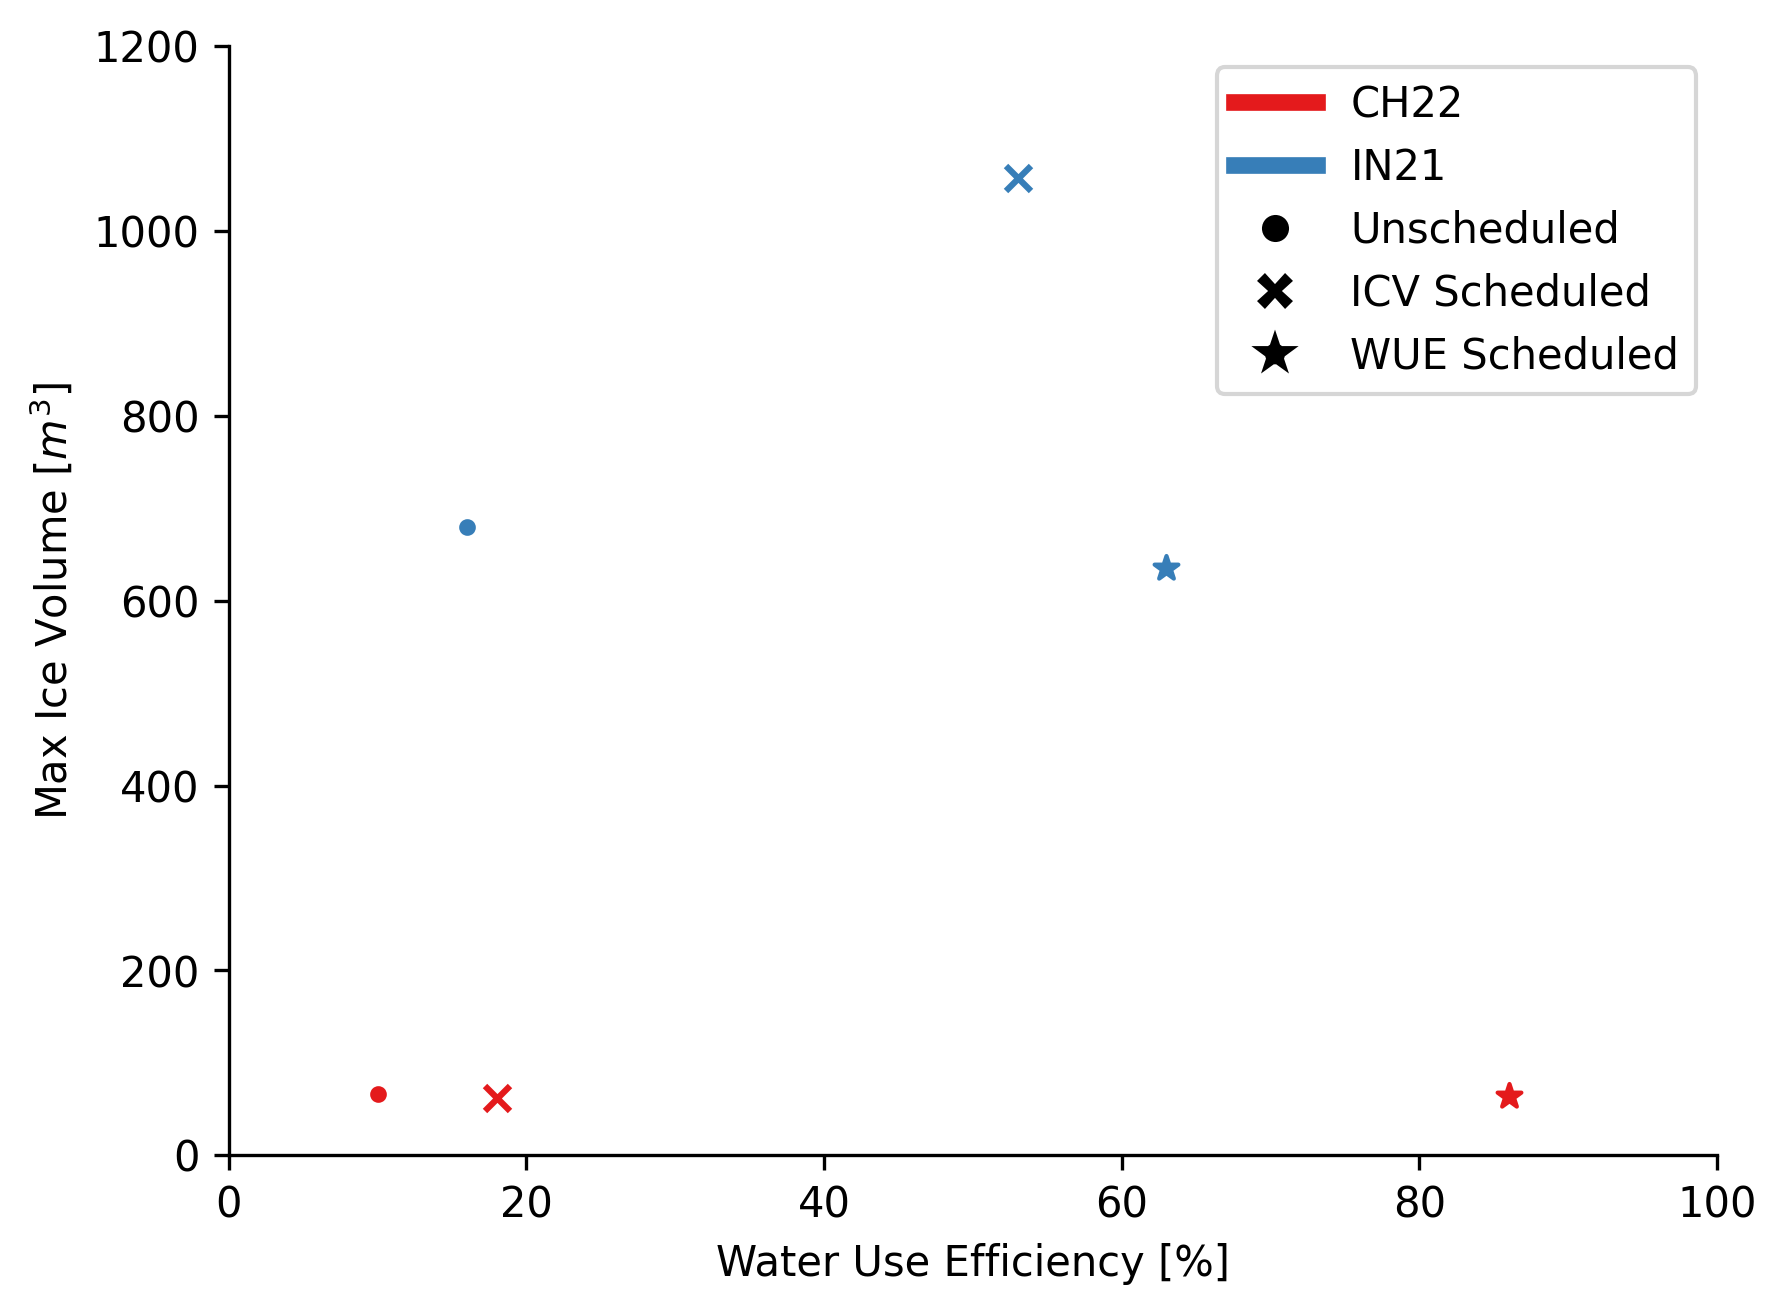
\includegraphics[width=12cm]{Figures/wue.png}

\caption{The maximum ice volume and water use efficiency estimated for AIRs constructed in different locations
(represented by colours) with different fountain scheduling strategies (represented by symbols). Experimental
values are highlighted by white circles and simulated values are highlighted by grey circles.  }

\label{fig:wue}
\end{figure*}

\subsection{Challenges of scheduling fountains}

Fountain freezing events limit the minimum discharge rate possible in scheduled fountains.  We assume the
minimum discharge rate that prevents fountain freezing events is 2 $l/min$. The model simulations revealed that
the nonzero median scheduled fountain discharge rate at the IN21 and CH21 AIRs were 13 $l/min$ and 2 $l/min$
respectively. Since the modelled scheduled discharge was lower than the minimum discharge rate for the Swiss
location, the automation system was programmed to overestimate the freezing rate as shown in Fig.
\ref{fig:simvsreal}. But model suggestions could be directly used in the case of the Indian location where
meteorological conditions and fountain spray radius favour a higher freezing rate. 

\begin{figure*}[t]
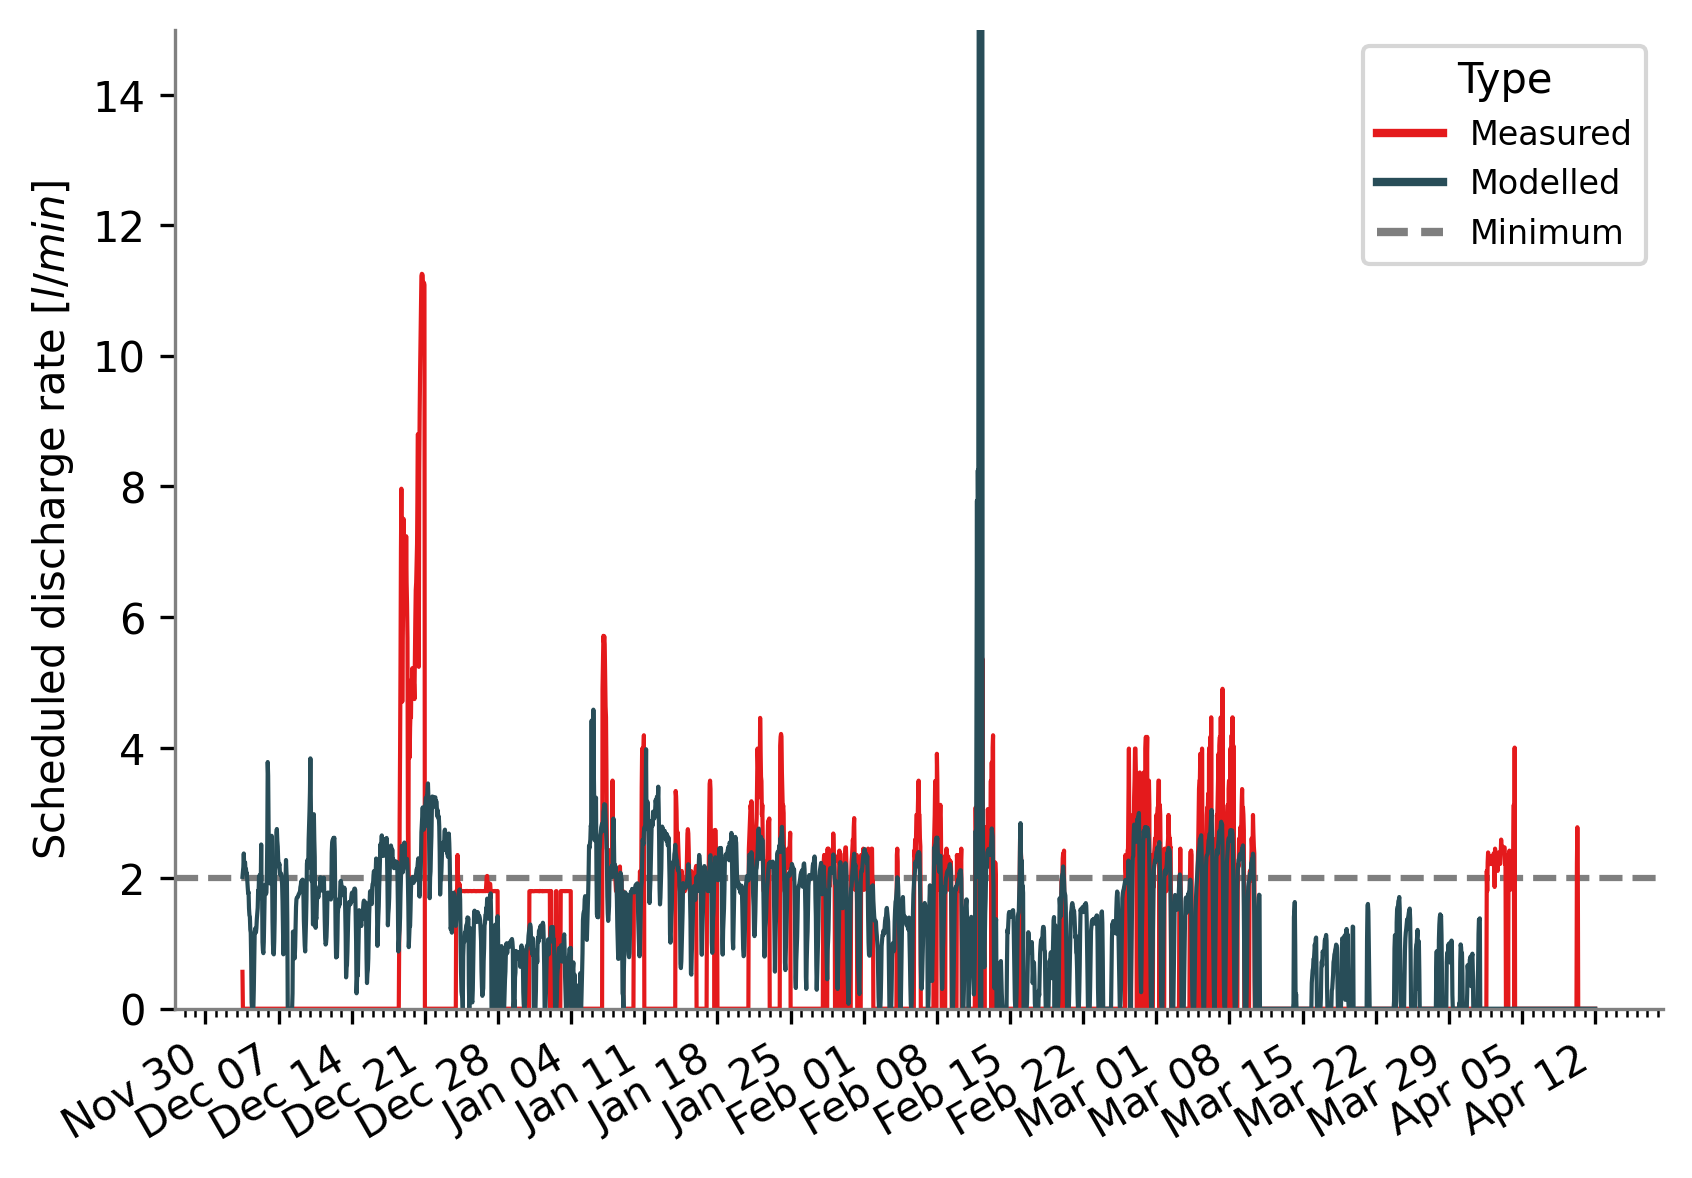
\includegraphics[width=12cm]{Figures/simvsreal.png}

\caption{ The discharge rate measured by the automation system (red line) and the modelled discharge rate of the ICV version
  of the simplified model (blue line) are compared. The dashed grey line represents the minimum discharge rate
that doesn't trigger fountain freezing events. }

\label{fig:simvsreal}
\end{figure*}

Fountain height increase events also trigger fountain freezing events. This is because the higher the fountain
the lower the gravitational pressure that drives the discharge rate. This was precisely why the unscheduled
fountain was interrupted by a fountain freezing event. This fountain freezing event was triggered almost
immediately after the fountain height was increased even though the fountain discharge had attained the critical
discharge rate as shown in Fig. \ref{fig:aws}. 

\subsection{Recommended fountain design}

Fountain design is another area where improvement is necessary. In the case of the CH22 experiment, the
scheduled and the unscheduled fountain produced a spray radius of 4.8 $m$ and 4.1 $m$ respectively. The
scheduled fountain produced a higher spray radius because of its lower aperture diameter. However, we suspect
that the lower aperture diameter also resulted in a higher pressure loss. In summary, an optimised fountain
design needs to decrease the aperture diameter while maintaining a reasonable pressure loss so that a higher
spray radius is achieved. 

\subsection{Recommended construction strategy}

We recommend three modifications to the traditional construction strategy to prevent fountain freezing events,
obtain higher ice volumes and lower water losses. Firstly, avoid fountain operation below the minimum fountain
discharge rate. Our study used a value of 2 $l/min$. However, this is likely to vary depending on the weather
conditions and the characteristics of the fountain and the pipeline used. It is recommended to set this value
based on observed fountain droplet trajectories in the construction site. Secondly, restrict maximum fountain
height based on the critical fountain discharge rate. Our study estimated the critical discharge rate to be 5
$l/min$. We believe this is a safe value to use for most fountains since most fountain designs have an aperture
diameter higher than aperture diameter used in our study. Once the maximum fountain height is achieved, another
AIR can be created to continue the construction process. Such a construction strategy would yield higher ice
volumes with lower risk of fountain freezing events. Thirdly, the maximum modelled discharge rate could be used
to set the mean discharge rate of unscheduled fountains. This will already yield a higher water use efficiency
without the need of sophisticated automation systems.

\conclusions

In this paper, an automated AIR construction strategy is presented and compared with a traditional strategy
using data collected in Guttannen, Switzerland.

The main purpose of this study was to quantify the influence of different fountain designs and scheduling
strategies on the water use efficiency and ice volumes of AIRs exposed to identical weather conditions. We found
that excessive fountain discharge rate not just increased the fountain wastewater production but also enhanced
the melting rate of AIRs mainly due to its surface albedo and surface temperature feedbacks. Furthermore, the
freezing rate of the scheduled fountain was also enhanced by its lower aperture diameter which contributed to
its higher spray radius. Therefore, the automated AIR was able to achieve a 34 \% higher maximum ice volume with
a five fold increase in the water use efficiency compared to the traditional AIR.

The automation system allows the easy handling of fountain scheduling implementation in any new location. The
possibility for changing the location and fountain metadata directly in the user interface allows tailoring the
fountain discharge rate according to the location's water supply and weather conditions. Furthermore, this
construction strategy reduces the occurence of fountain freezing events as it drains the pipeline outside
favourable weather windows and prevents fountain discharge rate to lower below a minimum threshold. Although,
the automation system increases installation costs, we believe use of such systems is warranted when considering
the reduced maintenance costs long term.

A simplified energy balance model compatible with the limited data availability of a new location was used to
produce two types of discharge rates favouring higher ice volumes and better water use efficiencies
respectively. Nevertheless, this model was able to capture more than 50 \% of the freezing rate variations
produced by the full energy balance model. Simulations comparing scheduled and unscheduled fountains show that
upto a two fold increase in water use efficiency is possible with the use of scheduled fountains.

Nevertheless, the real world application of this method is challenging. It is clear that if improvements are to
be achieved, future research must be devoted to improve fountain design in order to minimize their pressure
losses while increasing their spray radius.

\appendix

\section{Simplified energy balance model}


The model complexity was reduced through assumptions that optimise for the ice volume objective or the water use
efficiency objective. We define the freezing rate and melting rate as the positive and negative ice mass change
rate respectively. Assumptions are chosen based on whether they overestimate/underestimate the freezing rate.
Ice volume objective requires freezing rate to be overestimated whereas WUE objective requires freezing rate to
be underestimated. We describe these two kinds of assumptions applied on each of the energy balance components
below: 

\subsection{Surface Area $A_{cone}$ assumptions}

Determination of the surface area during the accumulation period is achieved by assuming a constant ice cone
radius equal to the fountain spray radius. The surface area scales the freezing rate of the AIR. Hence, for the
ICV objective we assume the maximum possible slope of 1 for the ice cone or in other words $h_{cone} = r_{F}$.
Therefore, area is estimated as:  

\begin{equation} A_{cone} =\pi \cdot r_{F}^2 \label{eq:Area} \end{equation}

Similarly, for the WUE objective, the area of the conical AIR is approximated to the area of its circular
base. Therefore, area is estimated as:

\begin{equation} A_{cone} =\sqrt{2} \cdot \pi \cdot r_{F}^2 \label{eq:Area} \end{equation}

\subsection{Net shortwave radiation \texorpdfstring{$q_{SW}$}{Lg} assumptions}
\label{sec:SW}

The net shortwave radiation $q_{SW}$ is computed as follows:

\begin{equation} 
q_{SW} = (1- \alpha) \cdot ( SW_{direct} \cdot f_{cone} + SW_{diffuse})
\label{eqn:SW} 
\end{equation}

where $\alpha$ is the albedo value ; $SW_{direct}$ is the direct shortwave radiation; $SW_{diffuse}$ is the
diffuse shortwave radiation and $f_{cone}$ is the solar area fraction.

The data requirement was reduced by estimating the global shortwave radiation and pressure directly using the
location's coordinates and altitude through the solar radiation model described in
\citet{holmgrenPvlibPythonPython2018}. The algorithm used to estimate the clear-sky global radiation is
described in \citet{ineichenBroadbandSimplifiedVersion2008}.  

The diffuse and direct shortwave radiation is determined using the estimated global solar radiation as follows:

\begin{equation}
\begin{split}
  SW_{diffuse} &= cld \cdot SW_{global}\\
  SW_{direct} &= (1-cld) \cdot SW_{global}
\end{split}
\end{equation}

where $cld$ is the cloudiness factor. $cld$ is assumed to be 1 and 0 for the WUE and ICV objective
respectively.

We ignore the variations in the albedo and assume it to be equal to snow albedo and ice albedo for the ICV and
WUE objective respectively.

The solar area fraction $f_{cone}$ of the ice structure exposed to the direct shortwave radiation depends on the
shape considered. It is computed as

\begin{equation}
		f_{cone} =\frac{(0.5 \cdot r_{cone} \cdot h_{cone}) \cdot cos \theta_{sun} +(\pi \cdot
			{(r_{cone})}^2/2) \cdot sin \theta_{sun} }{\pi \cdot r_{cone} \cdot ({(r_{cone})}^2+{(h_{cone})}^2)^{1/2}}\\
\end{equation}

For the ICV objective, since we assume the slope of the cone to be 1, $f_{cone}$ is determined as follows:

\begin{equation}
		f_{cone} =\frac{ cos \theta_{sun} + \pi \cdot sin \theta_{sun} }{2\sqrt{2} \cdot \pi }
\end{equation}

Similarly, for the WUE objective, since we assume the slope of the cone to be negligible, we get:

\begin{equation}
		f_{cone} =\frac{ sin \theta_{sun} }{2 }
\end{equation}

\subsection{Net Longwave radiation \texorpdfstring{$q_{LW}$}{Lg} assumptions} \label{sec:LW}

We assume $T_{ice} = 0 \degree C$ in order to determine outgoing longwave radiation. Since it is challenging to
contrain the minimum ice temperature, we maintain this assumption for both our objectives. However, in order to
estimate atmospheric emissivity we again assume $cld$ to be 1 and 0 for the WUE and ICV objective respectively.

\subsection{Turbulent fluxes assumptions} \label{sec:Qs}

Turbulent fluxes estimation depend on the slope of the cone through the $\mu_{cone}$ parameter. As suggested 
by \citet{oerlemansBriefCommunicationGrowth2021}, we can estimate this parameter as follows:

\begin{equation}
  \mu_{cone} =1 + s_{cone}/2
\end{equation}

Hence, the $\mu_{cone}$ parameter takes values of 1.5 and 1 for the ICV and WUE objective respectively.  Since
turbulent fluxes impact both the freezing and the melting rates, this assumption may not favor the corresponding
objectives for certain sites.

\noappendix 

\bibliographystyle{copernicus}
\bibliography{zot_refs.bib}

\end{document}
